\section{Correction Prescribed by the Identity}
\label{sec:method}

Theorem~\ref{thm:bias_identity} identifies per-subgroup misclassification deviation as the bias source; the natural correction is per-subgroup confusion matrix inversion.
This correction (EC-HTE) proceeds in three stages: estimate per-subgroup confusion matrices via hierarchical Bayes, invert them to correct observed outcome moments, and propagate correction uncertainty into downstream causal estimators.
The complete procedure is summarized in Algorithm~\ref{alg:echte} and illustrated in Figure~\ref{fig:method_overview}.

\begin{algorithm}[t]
\caption{EC-HTE: Error-Corrected HTE}
\label{alg:echte}
\begin{algorithmic}[1]
\Require $\{(Y_i, W_i, \hat{Z}_i, X_i)\}_{i=1}^N$; expert labels $\{Z_j^*\}_{j=1}^{n_{\text{expert}}}$; subgroup map $S$
\Ensure Corrected CATE estimates $\hat{\tau}(z)$ with CIs
\Statex
\State \textbf{Check:} $n_{\text{expert}} \cdot P(Z_{\min}) / K \geq 25$ and $\max_s \pi_s < 0.5$
\Statex
\State \textbf{Step 1: Per-subgroup CMs (hierarchical Bayes)}
\State $\alpha_0 \gets \arg\max_\alpha \prod_s p(\text{data}_s \mid \alpha, \hat{C}_{\text{global}})$
\For{$s = 1, \ldots, K$}
    \State $\hat{C}_s[j,k] \gets (n_{s,jk} + \alpha_0 \hat{C}_{\text{global},j,k}) / (n_{s,j\cdot} + \alpha_0)$
\EndFor
\State \textbf{Step 2: Stratified inversion}
\For{$s = 1, \ldots, K$}
    \If{$\kappa(\hat{C}_s) > 100$} $\hat{C}_s \gets \hat{C}_{\mathrm{global}}$ \Comment{$\kappa$-guard}
    \EndIf
    \State $\tilde{\boldsymbol{\mu}}_s \gets \hat{C}_s^{-1} \hat{\boldsymbol{\mu}}_s$
\EndFor
\State \textbf{Step 3: Downstream estimation}
\State Feed $\tilde{\boldsymbol{\mu}}_s$ into CausalForestDML (honest splitting)
\State $\mathrm{se}_{\mathrm{adj},i} \gets \sqrt{\mathrm{diag}(\hat{C}_{S_i}^{-1}\, \mathrm{diag}(\mathrm{se}_i^2)\, \hat{C}_{S_i}^{-\top})}$
\end{algorithmic}
\end{algorithm}

\begin{figure*}[t]
\centering
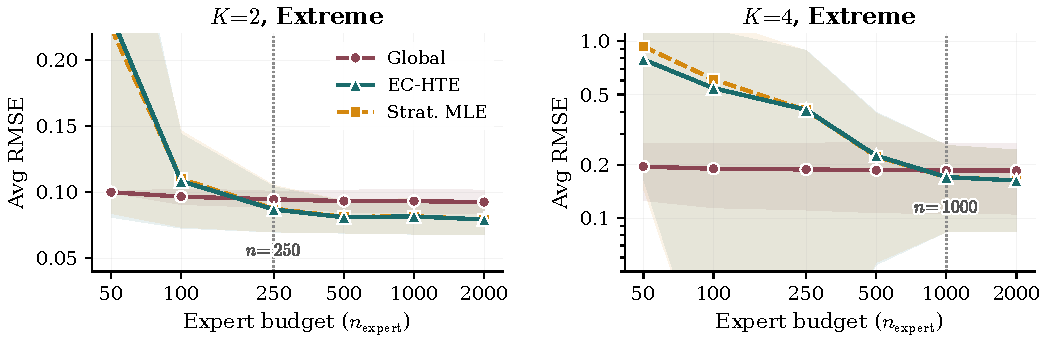
\includegraphics[width=\textwidth]{figures/fig4_budget_compact.pdf}
\caption{RMSE vs.\ expert budget under extreme heterogeneity. Crossover at $n{=}250$ ($K{=}2$) and $n{=}1000$ ($K{=}4$, $\Delta\tau{=}0.3$); under the Table~\ref{tab:main_results} DGP, $K{=}4$ crossover is lower ($n{\approx}500$). Shaded bands: $\pm 1$ SD. Full grid in Appendix~\ref{app:budget}.}
\label{fig:budget_compact}
\end{figure*}

\subsection{Hierarchical Bayes Confusion Matrix Estimation}

We place a Dirichlet-Multinomial hierarchical model over $\{C_s\}_{s=1}^K$, estimating the full $J \times J$ matrix per subgroup (no symmetric-error assumption).
Each row $j$ of $C_s$ has prior $\text{Dir}(\alpha_0 \cdot \hat{C}_{\text{global},j})$, where $\alpha_0 > 0$ is a shared concentration parameter estimated via empirical Bayes (marginal likelihood maximization; $<$5ms; MCMC alternative in Appendix~\ref{app:mcmc}).
We place a $\mathrm{Gamma}(3, 1)$ hyperprior on $\alpha_0$, robust to $2\times$ perturbation (Appendix~\ref{app:hyperprior}).
Large $\alpha_0$ pulls estimates toward $\hat{C}_{\text{global}}$; small $\alpha_0$ allows subgroup-specific rates to dominate.
The key design choice is hierarchical partial pooling rather than independent per-subgroup estimation: when expert labels are scarce ($n_{\text{expert}} / K < 100$), per-subgroup maximum likelihood estimation (MLE) suffers high variance from small cell counts, while global pooling discards the heterogeneity that Theorem~\ref{thm:bias_identity} identifies as the bias source.
Hierarchical Bayes (HB) outperforms stratified MLE in 87.5\% of configurations (Section~\ref{sec:ec_hte_eval}).

\subsection{Subgroup-Stratified Correction}

Given posterior mean confusion matrices $\hat{C}_s$, we correct observed outcome moments per subgroup by matrix inversion:
\begin{equation}
\tilde{\boldsymbol{\mu}}_s = \hat{C}_s^{-1} \cdot \hat{\boldsymbol{\mu}}_s,
\end{equation}
where $\hat{\boldsymbol{\mu}}_s = [\hat{\tau}_{\text{obs}}(0, s),\, \hat{\tau}_{\text{obs}}(1, s)]^\top$ collects the observed conditional outcome moments in subgroup $s$.
Invertibility requires $\pi_s \neq 0.5$ (A4); Laplace smoothing and a $\kappa$-guard ($\kappa(\hat{C}_s) > 100 \to$ fallback to $\hat{C}_{\mathrm{global}}^{-1}$; threshold ablation in Appendix~\ref{app:kappa_ablation}) ensure finite-sample stability.
All 11 tested LLM--dataset combinations fall in $\kappa \in (1.25, 3]$ with coverage $\geq$93\% (Appendix~\ref{app:kappa_analysis}).
Global correction applies $\hat{C}_{\mathrm{global}}^{-1}$ uniformly, introducing the $\delta_s \cdot \Delta\tau$ bias of Theorem~\ref{thm:bias_identity}; subgroup-stratified correction eliminates this at the cost of higher variance (Appendix~\ref{sec:budget}).

\subsection{Downstream Integration}

Corrected covariates are fed into CausalForestDML~\cite{wager2018causal} with honest splitting; bias corrections propagate as weighted averages of per-subgroup corrections ($R^2 > 0.97$ across 520 configurations; Appendix~\ref{app:bootstrap_se}).
Standard errors are adjusted via $\text{se}_{\text{corrected},i} = \sqrt{\text{diag}(\hat{C}_{S_i}^{-1}\, \text{diag}(\text{se}_i^2)\, \hat{C}_{S_i}^{-\top})}$; below $n_{\text{expert}}/K < 50$, a bootstrap ($B{=}100$) maintains $\geq$95\% coverage (Appendix~\ref{app:bootstrap_se}).

\paragraph{PPCI composition.}
EC-HTE corrects covariate misclassification; PPCI~\cite{sui2026ppci} corrects outcome-side error. Under both error types, composition reduces $|\text{bias}|$ from 0.179 to 0.007 (Appendix~\ref{sec:ppci}).